\documentclass{csfyp}
\usepackage{graphicx}
\usepackage{enumitem} %for {enumerate}[nolistsep]
\usepackage{titlesec} %for titlespacing
\usepackage{pgfgantt} %for Gantt chart

\titlespacing*{\section}{0pt}{0.4\baselineskip}{\baselineskip}
\titlespacing*{\subsection}{0pt}{0.4\baselineskip}{\baselineskip}

\titleformat*{\section}{\large\bfseries}
\titleformat*{\subsection}{\normalsize\bfseries}

\title{The Malta Human Genome Project \\
  \large Progress Report}

\author{Sara Ann Abdilla (188396M)}
\supervisor{Dr Jean-Paul Ebejer}
\date{December 2016}

\begin{document}

\pagenumbering{roman} 
\tableofcontents
\newpage
\listoffigures
%\listoftables

%\maketitle
\newpage

\pagenumbering{arabic} 
\setcounter{page}{1}


\begin{abstract}
Human genomes are being globally assembled in order to aid in medical diagnosis, forensic research, genealogy and bioinformatics among other areas.  While many countries have already had a reference genome constructed for their population, Malta is still in the process of accomplishing this - a National Maltese Human Reference Genome.  In this dissertation, we propose to build computational algorithms for the visualisation and analysis of DNA by developing a compression tool and a sequence aligner as deliverables, with the option of also producing a genome browser which would involve data visualisation capabilities.
\end{abstract}


\section{Introduction}\vspace{-2ex}
\label{s:intro}

Over the years, there has been an increase in sequencing of human genomes in order to identify genetic diseases.  This procedure is aided by a reference genome which is considered as a representative sample of a population's set of genes or DNA (to which individual's DNA sequences can be compared against)~\cite{omics}, where each individual's DNA corresponds to an arrangement of approximately 3 billion bases.  Each base can be one of four possible nucleotides: adenine, cytosine, guanine and thymine - oftenly referred to by the letters A, C, G and T respectively.  DNA (deoxyribonucleic acid) could be described as a model of biological life which encompasses genetic information/genes~\cite{aiBk, introgenom} - it is analogous to a storage device of genetic information.  

Genome assembly/sequencing technologies and projects are rapidly advancing and their costs are decreasing.  DNA variations and mutations may correlate to diseases so finding differences between a reference genome and the genome of a patient afflicted with a disease has important implications for medical diagnosis and treatment~\cite{think} as genes are hereditary from one generation to the next.  Examples of these genome projects include the 100,000 Genomes Project in the UK and the International Cancer Genome Project~\cite{bwtransform, refcompression, popgen}.

The University of Malta is developing a National Maltese Human Reference Genome whereby whole genome sequencing of certain Maltese DNA samples (provided by the Malta BioBank) will be performed.  The American human genome sequencing facility Complete Genomics, which was founded in 2006, is a partner in this project.  This development is required in order to identify any DNA mutations which are predominant in the Maltese population.  Comparing the provided Maltese DNA samples with any other human reference genome, for example with a Japanese reference genome, would not provide any accurate results as Maltese and Japanese people have a diverse gene pool.  This is due to the fact that both populations are descendant from diverse civilisations, so both of their evolutionary histories are different.  This same fact can be said for any two distinct nationalities, thus providing incentive for a Maltese reference genome.  

A read is a nucleotide sequence which is gathered by sequencers from cloned fragments of the genome as depicted in Figure 1.  This is done as DNA sequencing technologies are unable to read whole genomes, but sequencing reads pose no problems.  

\begin{figure}[h!]
  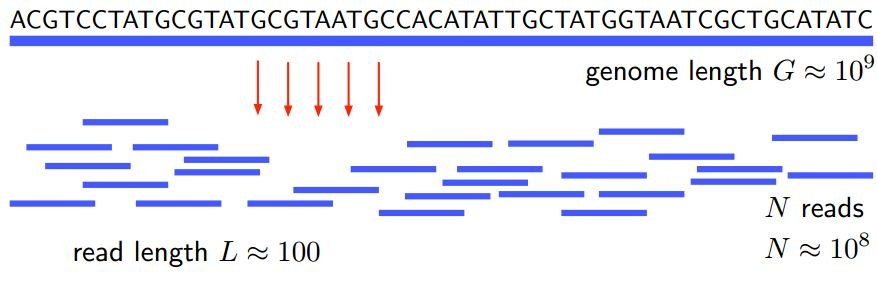
\includegraphics[width=\linewidth, height=120]{dnareads.jpg}
  \caption{DNA sequencing reads}
  \label{fig:reads}
\end{figure}

The problem of aligning genomes comes into play here.  The reading of an individual's DNA shows the likeliness of that person developing a disease, but the reading of a nation’s DNA shows why that population is more likely to develop a disease~\cite{think}.  In order to accurately and efficiently match alignments between a human reference genome and the respective DNA sequencing reads, different algorithms must be applied.  The most common aligners use Burrows-Wheeler Transform~\cite{bwtransform, cgreads} but there are multiple other algorithms; see section 2.2 for more details.  

Thus, computation wise, tools which deal with DNA analysis and visualisation need to be constructed in order to aid in this endeavour.  These developments are only possible after the alignment of a set of sequencing reads against a reference genome is completed.  

\subsection{Motivation}\vspace{-2ex}
While the National Maltese Human Reference Genome is gradually being developed, analysis tools for it are still in a dormant phase.  This project will mainly focus on constructing these DNA analysis and visualisation tools so it would be desirable to begin implementing them to ensure the success of the entire Malta Human Genome Project (MHGP).   

\subsection{Why is this a non-trivial problem?}\vspace{-2ex}
A major problem with genome projects is their efficiency with regards to their accurate alignment.  When aligning a set of sequencing reads against a reference genome, different alignment methods will produce diverse performance especially when single and parallel process execution is considered.  The more efficient the produced tools are, the easier it is to analyse and visualise the DNA.     


\section{Background Research and Literature Review}\vspace{-2ex}

The development of a genome assembly technology consists of multiple stages; the main ones being genome compression, sequence alignment, alignment visualisation and genome browser construction (successively).  The following points detail some research which has already been conducted in these areas.

\subsection{Genome Compression Tools}\vspace{-2ex}
Genomes, particularly human ones, consist of a large amount of data - approximately 3,000 Mb (megabase pairs).  For this reason, in order to efficiently analyse them, said genomes are compressed using various methods.  

For example, Chen et al devised the lossless {\textit{GenCompress}} algorithm which implements certain established compression algorithms such as Lempel-Ziv~\cite{gencompress}, a variable-to-fixed-length code which parses the input sequence into non-overlapping DNA fragments of differing lengths while also constructing a dictionary of the fragments observed.    By analysing approximate matches based on the evaluated edit distances, it was found that such a method not only achieves the best compression ratio but also finds common sections in DNA sequences~\cite{gencompress}.  Another example would be the lossless reference-based compression algorithm devised by Fritz et al~\cite{refcompression}.  It implements established components such as Golomb codes, optimal prefix codes (i.e. no codeword is a prefix of any other codeword in the relative system), and De Bruijn graphs, directed graphs symbolising overlaps between sequences, and was found to be quite efficient for read alignments similar to the reference genome.  Other known algorithm are {\textit{Biocompress-2}} and {\textit{Cfact}}~\cite{gencompress} along with {\textit{DNACompress}} and {\textit{ DNAZip}}~\cite{refcompression}.          

\subsection{Read Alignment Tools}\vspace{-2ex}
Next-Generation Sequencing (NGS) technologies are evolving rapidly and to keep up with this evolution, multiple read aligners are being produced; the most known being BWA, Bowtie, Soapv2, MAQ, BOAT, SHRiMP2 for the NGS platforms Illumina, Roche454 and ABI SOLiD~\cite{bwtransform, popgen, cgreads}.  These sequencers are given such importance due to the fact that genomic analysis would prove to be impossible without them.  Reference genomes are produced using them so without this basic building block, no initial analysis can even commence.     

The majority of read aligners implement Burrows-Wheeler Transform (BWT - permutes the bases of a sequence into another sequence) but there are also those which use FM-indexing (finds the number of occurrences of a read within a genome along with each occurrence's position), Needleman-Wunsch (finds similar regions between nucleotide sequences by comparing DNA fragments of differing lengths), and Smith-Waterman (a variation of Needleman-Wunsch) algorithms~\cite{bwtransform, popgen, cgreads}.  All these mentioned aligners are quite efficient relative to the task they are given; for example, while some aligners may be more efficient with short reads, others may be more efficient with longer reads~\cite{companalys, compalign}.  Other known algorithms which assist in approximate read mapping are the Hamming distance as well as the Levenshtein distance.  The Hamming distance method evaluates the number of mismatches between two sequences with regards to substitutions while the Levenshtein/Edit distance method evaluates the number of mismatches between two sequences with regards to substitutions, insertions and deletions.  These are not as commonly used due to their relative shortcomings.  Both have an inefficient time complexity and the Hamming distance algorithm can even prove to be inaccurate as it only considers substitutions, unlike the Levenshtein distance which not only considers substitutions but also insertions and deletions.  

\subsection{MapReduce Framework}\vspace{-2ex}
MapReduce is a parallel programming model which processes and generates large datasets whereby {\textit{Map}}, by definition, takes an input pair and returns a set of intermediate key-value pairs to {\textit{Reduce}} which takes an intermediate key and a set of values for the respective key and merges them to return a smaller set of values.  It was originally produced by Google to query trillions of web pages, but it has started to be included in multiple other areas which also involve large datasets due to its parallelisation feature~\cite{mapreduce}; i.e. simultaneous process execution.    

This model was used as a framework for read alignment by Menon et al.~\cite{mapredgen} due to its parallelisation, by incorporating suffix arrays (sorted arrays of all the suffixes of a sequence), BWT and cloud computing in their implementation.  Unfortunately, the current implementation of this framework is not working due to the multiple advances in sequencing technologies.              

\subsection{Genome Browsers}\vspace{-2ex}
Genome browsers are graphical interfaces which are used for analysis in conjuction with genomic databases.  They display the information found such that individuals are able to not only browse the stored genomes but also to visualise them, leading to easier data seaching and analysis.  Most browsers are web-based applications which allow certain customisations according to the user's requirements, but stand-alone browsers exist as well~\cite{webbrowser, genericbrowser}.  An example of a web-based genome browser is {\textit{GBrowse}} which was constructed by Stein et al.~\cite{genericbrowser}. 
 
Genome browser construction has an intricate development process.  Fortunately, many genome browser frameworks have already been constructed such as the most popular {\textit{GBrowse}} (which was mentioned previously) as well as {\textit{Ensembl}}, {\textit{JBrowse}} and {\textit{LookSeq}} among others.  It should also be noted that there are two types of web-based genome browsers, multiple-species and species-specific browsers~\cite{webbrowser}.  As this project deals with a human genome, a species-specific browser will be implemented.  Following the Generic Model Organism Database (GMOD) project, there are multiple open-source tools for this type of browser; {\textit{GBrowse}}, again, being one of the most used frameworks~\cite{webbrowser}.              

\subsection{Gaps in Current Research}\vspace{-2ex}
As mentioned in section 2.3, the read aligner which implements the MapReduce framework is not working.  We will therefore be creating our own implementation with the use of this framework to parallelise the system (i.e. contribution to field).     
     

\section{Aims and Objectives}\vspace{-2ex}

The aim of this project is to develop algorithms and build tools for the analysis of sequenced genomes from the Malta Human Genome Project.  The research areas studied are bioinformatics, big data, data storage, data visualisation and data analysis among others.  The main objectives of the system are as follows:

\begin{enumerate}[nolistsep]

   \item The compression of a reference genome such as that done by Chen et al.~\cite{gencompress} and Fritz et al.~\cite{refcompression};

  \item The alignment of a reference genome against a number of sequencing reads such as that done by Lee et al.~\cite{cgreads} and Li et al.~\cite{bwtransform};

  \item The use of the MapReduce framework such as that done by Menon et al.~\cite{mapredgen};

\end{enumerate}

Depending on project and time constraints, the construction of a genome browser could also be completed using novel and established components (such as that done by Stein et al.~\cite{genericbrowser}) in order to reference and visualise DNA for comparitive genomics and to analyse DNA mutations.


\section{Methods Development}\vspace{-2ex}

This section details the components which have been implemented along with a description of future plans.

\subsection{Genome Compression}\vspace{-2ex}
The genome compression method implemented compresses the acquired human genome, having a size of approximately 3GB, into a binary file by means of integers (each integer being of length 4 bytes).  Each nucleotide base is assigned two bits to represent it as there are only 4 possible bases. Chen et al. used the same deduction when developing {\textit{GenCompress}~\cite{gencompress}.  The implementation used acheived a compression rate of 70\%, from roughly 3GB to 1GB.  The method chosen was also observed to be accurate after some decoding tests took place.        

\subsection{Sequence Alignment}\vspace{-2ex}
Four possible alignment methods were then taken into consideration; the number of human sequencing reads being 28,094,847 with each read having a length of 60 bases; i.e. 30 base-pairs/bp.  The Hamming distance and the Levenshtein/Edit distance methods both return a measure of the similarity between two sequences,  {\textit{k}-mer indexing evaluates all the possible subsequences of a sequence of length {\textit{k} into an index and the most frequently used FM-indexing evaluates all the possible subsequences of a sequence using BWT into an index.  BWT transforms a base sequence into multiple runs having similar bases.  

These aligners were first implemented and tested on string inputs; i.e. on an uncompressed genome of marginally less size than the human genome to confirm their applicability.  Some of these functions were then converted in order to instead support integer inputs due to the previously mentioned genome compression.  This was done by using bitwise operations and by finding any patterns in the integer sequence; i.e. any repetitive integers or pairs of integers or triples and so on in the compressed reference genome.        

\subsection{Alignment Visualisation}\vspace{-2ex}
The data visualisation tool's initial construction is based on {\textit{Tkinter}}, Python's standard Graphical User Interface (GUI) package.  The result is a depiction of the reads aligned with the genome, with lines representing the position and length of each alignment/match.  As of now, its interactivity is in the form of clicking a line at a certain position to output the offset of the match at the point of clicking.     

\subsection{Future Plans}\vspace{-2ex}
As for future developments, firstly, the read alignment methods need to all be converted to support integer inputs (due to the genome compression applied) and then compared in order to deduce the most efficient one in terms of the match rate with the corresponding time taken.  An improvement on the BWT implementation will be done by incorporating the MapReduce parallel programming model, as described by Menon et al.~\cite{mapredgen}, in order to accelerate the transformation.  

Secondly, the data visualisation tool needs to be further refined; i.e. become more interactive in terms of genome analysis.  This could be accomplished by outputting the DNA mutation found at the point of clicking instead of just the offset, or perhaps even both.       

Optionally, depending on the project's time constraints, the genome browser tool could also be constructed using the established technologies (described in section 3) for efficient comparitive genomics; the visualisation tool being incorporated in this.  Each method developed will be analysed and compared to deduce the most feasible implementation.   


\section{Evaluation}\vspace{-2ex}

The main evaluation techniques proposed are as follows:

\begin{enumerate}[nolistsep]

  \item	Comparitive review of the developed read aligner with the other developed aligners and with existing methods by comparing match rates with the corresponding time taken;

  \item Comparitive review of the MapReduce read aligner (parallel process execution) against a single process execution;  

  \item Review of the developed human genome visualisation tool by testing that its interface is easily understood by most users by, for example, checking that the data is output in a clear manner;

  \item Possible comparitive review of the constructed genome browser by referencing DNA and analysing DNA mutations followed by comparison of results with existing methods.

\end{enumerate}


\section{Deliverables}\vspace{-2ex}

\begin{enumerate}[nolistsep]

  \item The Final Year Report which will include all the relevant background information required to understand said project, a detailed explanation and the evaluation results; 

  \item The implementation (code) of the designed and developed system;

  \item The documentation which will explain to the users how the system should be employed; i.e.\ a user manual. 

\subsection{Project Timeline}\vspace{-2ex}

The milestone schedule is represented in the following Gantt chart: \\

\tikzset{every picture/.style={yscale=0.8,transform shape}}
\noindent\resizebox{\textwidth}{!}{
\begin{ganttchart}[
    hgrid=true,
    vgrid=true,
    bar/.style={fill=black!50}
]{1}{30}
\gantttitle{2016--2017}{30} \\
\gantttitle{Sep}{3} 
\gantttitle{Oct}{3} 
\gantttitle{Nov}{3} 
\gantttitle{Dec}{3} 
\gantttitle{Jan}{3} 
\gantttitle{Feb}{3} 
\gantttitle{Mar}{3} 
\gantttitle{Apr}{3} 
\gantttitle{May}{3}  
\gantttitle{Jun}{3}\\
\ganttbar{Research \& Literature Review}{1}{12} \\
\ganttbar{Progress Report}{8}{11} \\
\ganttbar{Implementation}{4}{20} \\
\ganttbar{Evaluation}{20}{24} \\
\ganttbar{Documentation}{23}{27} \\
\ganttbar{Review Report}{24}{27} \\
\ganttbar{Presentation}{28}{29} \\
\ganttbar{Exhibition}{30}{30}
\end{ganttchart}
}

\end{enumerate}


%\bibliographystyle{alpha}
\bibliographystyle{ieeetr}
\nocite{*}
\begingroup
    \setlength{\bibsep}{10pt}
    \setstretch{0.85}
    \bibliography{references}
\endgroup
%\bibliography{references}

\end{document}
